\chapter{Introduzione al contesto di applicazione del progetto}

\section{Concetto base della regata}
Una \textbf{regata} è una competizione tra imbarcazioni che possono essere a remi oppure a vela. Tale competizione consiste nel completare, una o più volte, un percorso prestabilito tramite un \textit{bando di regata}\cite{regata_costiera}. La partenza delle imbarcazioni prevede un conto alla rovescia preceduto da dei segnali acustici (sirene) e visivi (bandiere o nel caso di competizioni notturne, segnali luminosi). Le imbarcazioni devono effettuare un percorso prestabilito da diverse boe che sono state posizionate in diversi punti del campo della regata. Il \textit{campo della regata} rappresenta il luogo in cui viene svolta la competizione. L'arrivo è contrassegnato da una linea immaginaria tracciata da due boe o da un cordino teso tra due sostegni galleggianti. 

\section{Regata costiera}
Il campo della regata in questa categoria di competizioni può essere sia il mare che i laghi e i corsi d'acqua dolce, purché siano sufficientemente ampi. Nel contesto in cui verrà utilizzata l'applicazione, il campo della regata è il mare \cite{vela_sport}.

Il tracciato della regata è costituito dal posizionamento dei \textbf{waypoint} nel campo della regata, ovvero dei punti definiti nello spazio (coordinate geografiche) che rappresentano le posizioni relative ad ostacoli (possono essere boe o barche). È di fondamentale importanza posizionare correttamente i waypoint, in quanto un errato posizionamento di essi può generare degli scompensi durante la competizione. Tuttavia, durante la regata possono verificarsi delle condizioni non previste, in particolare condizioni meteo inaspettate, come del vento forte, che possono spostare fisicamente le boe nel campo di regata. Conseguentemente a questo fatto, i partecipanti hanno delle rotte differenti rispetto alla posizione effettiva della boa.

\section{Barca a vela}
Il lavoro svolto in questa tesi va a contribuire ad un progetto di ricerca dell'Università degli Studi di Udine: \textbf{UniUD Sailing Lab}. È un progetto di ricerca del Dipartimento Politecnico di Ingegneria e Architettura in cui viene utilizzata una barca a vela da regata. La barca \textbf{William B} è un modello \textit{Archam-bault A35} ed è dotata di sensori ed hardware in grado di raccogliere e memorizzare dati in tempo reale sulla navigazione per il controllo e la gestione delle attività di bordo.
L'applicazione mobile va a fornire un supporto all'equipaggio per le decisioni da prendere e le strategie da applicare durante la competizione.
\begin{figure}
	\begin{center}
		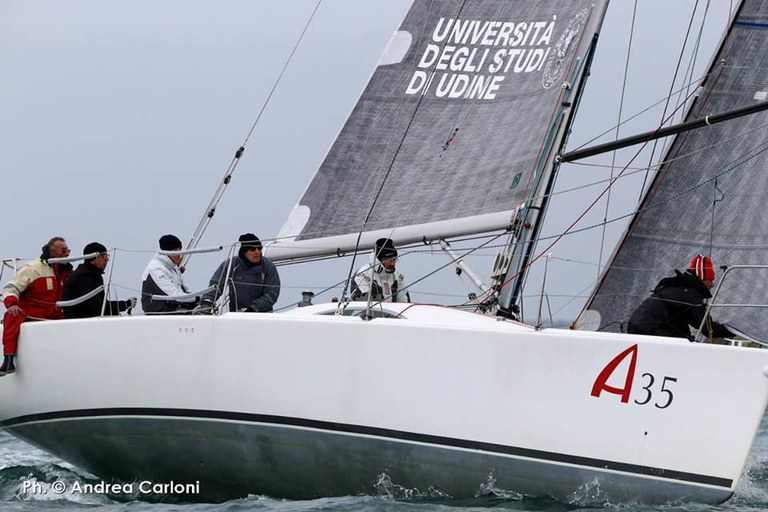
\includegraphics[scale=0.5]{william_b}
		\caption[Barca a vela Williab B]{Barca a vela da regata \textit{William B} \cite{william_b}}
		\label{figura:william_b}
	\end{center}
\end{figure}